\lecture{17}{04.18}
在三相点,$\Phi = 3, f = 0$ ,温度和压力都由系统决定
\begin{notation}
    热力学温度1K被定义为水的三相点温度的$\frac{1}{273.16}$
\end{notation}
如图,在100kPa时,温度升高,依次经过固态、液态、气态,及冰-水-水蒸气,如果在100摄氏度下,逐渐升高气压,从气态变为液态,这其中的自由度变化:
\begin{itemize}
    \item 第一个过程:$f = 2\to f = 1 \to f = 2\to f = 1\to f = 2$
    \item 第二个过程:$f = 2\to f = 1\to f = 2$
\end{itemize}
\begin{notation}
    冰点温度比三相点温度低0.01K,原因有:
    \begin{itemize}
        \item 外压增加,水的凝固点降低月0.0075K
        \item 水中溶解的空气形成稀溶液,溶质存在降低冰点约0.0025K
    \end{itemize}
\end{notation}
\subsection{超临界}%
\label{sub:超临界}
在液体和气体的交界处,如果温度足够高,会形成超临界流体,同时具有液体和气体的性质:
\begin{figure}[htpb]
    \centering
    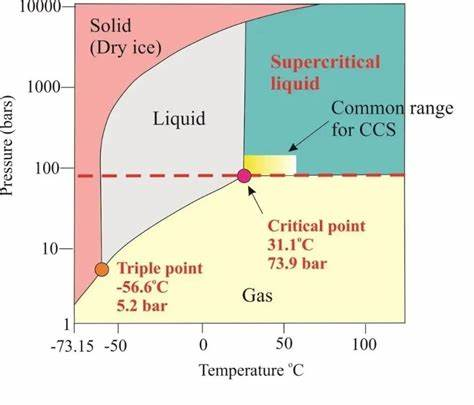
\includegraphics[width=0.8\textwidth]{./figures/二氧化碳相图.jpg}
    \caption{二氧化碳相图}
    \label{fig:-figures-二氧化碳相图-jpg}
\end{figure}
\begin{notation}
二氧化碳的超临界温度只有31.3摄氏度,且压力在100bar以内(7.38MPa),成本低、无污染、抗氧化、粘性低、无残留,因此SC-$\ce{CO_2}$ 是工业、食品、医药常用的超临界流体
\end{notation}
\subsection{完全互溶双液系统}%
\label{sub:完全互溶双液系统}
对于两组分系统,根据相率:
\[
    f + \Phi = C+2
.\]
$C=2, f=4-\Phi, \Phi\ge 1$,因此$f\le 3$。这三个变量通常为$T,p$ 和组成$x$ ,需要用三个坐标的立体图表示;保持一个变量为常量,截取横截面得到常用相图:
\begin{itemize}
    \item $p\sim x$ 图(最常用)
    \item $T\sim x$ (一般常用)
    \item $p\sim T$ (不常用)
\end{itemize}
\begin{figure}[htpb]
    \centering
    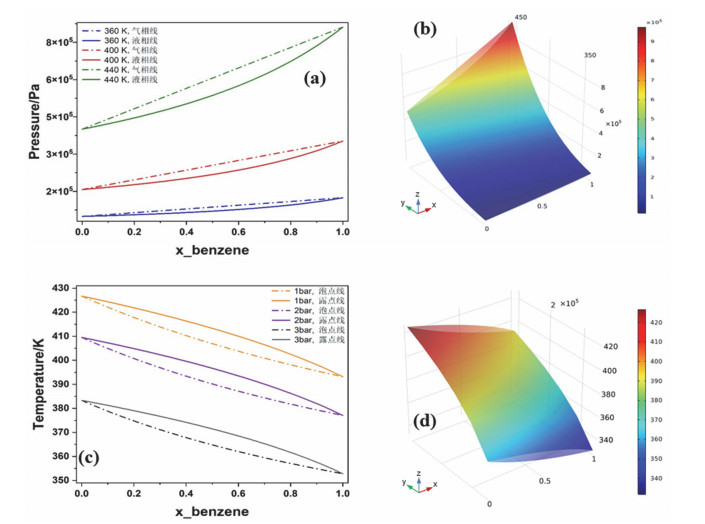
\includegraphics[width=0.8\textwidth]{./figures/三维相图.jpg}
    \caption{三维相图}
    \label{fig:-figures-三维相图-jpg}
\end{figure}
\subsubsection{\textit{p-x}图}%
\label{subsub:-textit-p-x-图}
根据拉乌尔定律:\[
    p_\text{A} = p^\star_\text{A} x_\text{A}\quad p_\text{B} = p_\text{B}^\star x_\text{B} = p_\text{B}^\star \left( 1-x_\text{A} \right)
.\]
总压:\[
    p = p_\text{A} + p_\text{B} = p_\text{B}^\star +\left( p_\text{A}^\star -p_\text{B}^\star  \right)x_\text{A}
.\]
当$x_\text{A} = 0$ 时,$p = p^\star _\text{B}$ ,反之$p = p^\star _\text{A}$ 
\begin{notation}
    对于包含气相:当平衡后,$y_\text{A} = \frac{p_\text{A}}{p}, y_\text{B} = 1-y_\text{A}$ ,带入得:\[
        y_\text{A} = \frac{p_\text{A}^\star x_\text{A}}{p_\text{B}^\star +\left( p_\text{A}^\star -p_\text{B}^\star  \right)x_\text{A}}
    .\]
\end{notation}
对于二组分系统(如图\ref{fig:-figures-三维相图-jpg}),其曲线为边界线,表示系统中一个新的相开始出现,由边界线(如气相线和液相线)围成的区域是两相平衡共存的区域
\subsubsection{\textit{T-x}图}%
\label{subsub:-textit-T-x-图}
可以从$p\sim x$ 图转为$T\sim x$ 图,也可以从实验绘制。
\begin{notation}
    杠杆规则: 在$T\sim x$ 图上:\[
        \frac{n\left( \text{l} \right)}{n\left( \text{g} \right)} = \frac{x_\text{g} - x_0}{x_0-x_\text{l}}
    .\]
    即:两相的量反比于他们到总组成点的距离(类似杠杆平衡原理)
\begin{figure}[ht!]
    \centering
    \incfig[0.5]{杠杆规则}
    \caption{杠杆规则}
    \label{fig:杠杆规则}
\end{figure}
\end{notation}
\begin{notation}
    最低恒沸混合物:混合物,改变压力时最低恒沸点温度改变,组成也随之改变,如含水乙醇(95\%)
\end{notation}
\begin{notation}
    精馏:通过分馏塔多次汽化、冷凝,使得低沸点物质越来越少
\end{notation}
